%%
%% This is file `esapub.tex',
%% generated with the docstrip utility.
%%
%% The original source files were:
%%
%% esapub.dtx  (with options: `manual')
%% ============================================
%% This is the manual describing the usage of
%%      esapub.cls
%% ============================================
%% Copyright 1999 Patrick W Daly
%% Max-Planck-Institut f\"ur Aeronomie
%% Max-Planck-Str. 2
%% D-37191 Katlenburg-Lindau
%% Germany
%% E-mail: daly@linmpi.mpg.de
%%
%% -------------------------------------------------
\documentclass[a4paper,twocolumn]{spaceDebrisC} % European paper
\pagestyle{empty}

% \bibliographystyle{alpha}
\bibliographystyle{apalike}

\usepackage{times}
\usepackage[numbers]{natbib}
\usepackage{graphicx}

\usepackage{bm} % for bold math
\usepackage{mathtools} % for \prescript
\newcommand{\vctr}[1]{\bm{#1}}
\newcommand{\unitv}[1]{\hat{\vctr{#1}}}
\newcommand{\preup}[1]{\prescript{#1}{}{}}
\newcommand{\rf}[1]{\mathcal{\MakeUppercase{#1}}}
\newcommand{\dcm}[1]{\left[\rf{#1}\right]}
\newcommand{\vrf}[2]{\preup{\rf{#1}}\vctr{#2}}
\newcommand{\mbar}[0]{\;\middle|\;}
\newcommand{\prf}[1]{\preup{\rf{#1}}}
\newcommand{\norm}[1]{\left\lVert#1\right\rVert}

\newcommand{\matcp}[1]{\left[#1 \times\right]}
\newcommand{\rthree}[0]{$\mathbb{R}^3$\:}
\newcommand{\sthree}[0]{$\mathbb{S}^3$\:}
\newcommand{\sothree}[0]{$SO_3$}
\newcommand{\pogslla}[0]{$32.900^\circ \textrm{ N}, -105.533^\circ \textrm{ W} \textrm{ }$}

\newcommand{\fighuge}[0]{1.0\textwidth}
\newcommand{\figbig}[0]{0.8\textwidth}
\newcommand{\figmed}[0]{0.6\textwidth}
\newcommand{\figsmall}[0]{0.4\textwidth}

\newcommand{\subfigmed}[0]{0.4\textwidth}
\newcommand{\subfigsm}[0]{0.29\textwidth}
\newcommand{\subfigbig}[0]{0.43\textwidth}

\DeclareMathOperator{\atantwo}{atan2}
\DeclareMathOperator{\fl}{floor}

\title{Optimal Light Curve Attitude Inversion with Measurement Noise: Two Case Studies}
\author{Liam Robinson}
\author{Carolin Frueh}
\affil{Purdue University, West Lafayette, United States, Email: \texttt{\{robin502, cfrueh\}$@$purdue.edu}}

\begin{document}

\keywords{Light curve inversion; Atitude estimation; Photometry; Inverse problems}

\maketitle

\begin{abstract}

Understanding the orientation and angular velocity state of active or passive human-made space objects is critical for many operations like long-term orbit propagation, aiding a mission, determining mission status, and active debris removal. Beyond low-Earth orbit, optical telescopes are used predominantly to track the space objects. Although this data is abundant, it is generally impossible to resolve even large satellites and rocket bodies in optical ground-based imagery due aperture size and atmospheric distortion. As a result, shape and orientation information is not available in any single image. But a measurement of the object's total brightness can still be obtained. Even if the object's shape and reflective properties are known, any given brightness measurement generally corresponds to infinitely many possible orientations. To constrain the solution space, the brightness can be tracked over time -- producing a sequence of measurements called a light curve. If the identity of the object is known, its attitude profile can be estimated from the light curve through a process known as light curve attitude inversion. Due to the natural and instrumental noise in the light curve, as well as symmetries in the observation geometry, there may be multiple attitude profiles which are equally likely to produce any given light curve.

In this work, we apply a light curve attitude inversion algorithm to real observations taken by the Purdue Optical Ground Station. Given an estimate of the shape and reflective properties of the object, our procedure searches the space of initial orientations, angular velocities, and inertia tensors to find initial conditions that produce light curves with low error compared to the observed values. Specifically, we estimate a full distribution for each candidate light curve and compute the likelihood of the observations being a sample from that distribution. To solve the optimization problem, we create a number of sampled candidate solutions, deterministically arranged throughout the solution space, and perform nonlinear optimization on each using the BFGS algorithm. This way, our optimization procedure reliably converges to all maximum likelihood estimates of the attitude state. Low-error minima are then clustered to identify families of nearby solutions with similar likelihood. The final output of our method is an array of the best solutions, ranked by their likelihood. Formulating the problem this way inherently accounts for the multiple classes of ambiguities resulting from the object and observation geometry, the physical constraints of torque-free rigid body motion, as well as the noise on the light curve.

To test the efficacy of this method, we perform attitude inversion on real observations gathered by the Purdue Optical Ground Station of an inactive GLONASS satellite and a rocket body. Solutions for the GLONASS case are analyzed to highlight the effect of observation geometry ambiguities, while the rocket body case highlights ambiguities introduced by the geometry of the object. Our noise model is validated against further real observations, confirming that all relevant noise sources have been accounted for and modeled accurately. We show that any significant lack of knowledge in the object shape or optical material properties causes the solution to rapidly degrade.

\end{abstract}

\section{Introduction}

test

\section{Inversion Method}

\begin{equation} \label{eq:nll_loss}
  f_\text{NLL}(\hat{\vctr{S}}, \vctr{S}) = \frac{1}{m}\sum_{k=1}^{m}\left[\ln\sigma_k + \frac{1}{2}\left(\frac{S_k - \hat{S}_k}{\sigma_k}\right)^2 \right].
 \end{equation}

\begin{equation}
  \vctr{x} = \begin{bmatrix} 
  p_1 & p_2 & p_3 & \omega_1 & \omega_2 & \omega_3 & \frac{J_y}{J_x} & \frac{J_z}{J_x}
  \end{bmatrix}^T.
 \end{equation}

\begin{align}
  \vctr{\dot{\sigma}} &= \frac{1}{4} \left[ \left(1 - \vctr{p} \cdot \vctr{p}\right) + 2\vctr{p} \times \vctr{\omega} + 2 \left(\vctr{\omega} \cdot \vctr{p} \right)\vctr{p} \right] \label{eq:mrp_kde} \\
  \vctr{\dot{\omega}} &= J^{-1} \left[ \left(J \vctr{\omega}\right) \times \vctr{\omega} + \vctr{M}\right] \label{eq:rbtf_dynamics}
\end{align}

\begin{equation}
  \vctr{p}'' = \frac{\left(1-\norm{\sigma'}^2\right)\vctr{p} - \left(1-\norm{\vctr{p}}^2\right)\vctr{p}' - 2\vctr{p} \times \vctr{p}'}{1 + \norm{\sigma'}^2 \norm{\vctr{p}}^2 + 2\vctr{p}' \cdot \vctr{p}},
\end{equation}

\begin{equation} \label{eq:angle_error}
  \theta = 4 \tan^{-1} \left( \norm{\vctr{p}''} \right).
\end{equation}

\begin{figure}[ht]
  \centering
  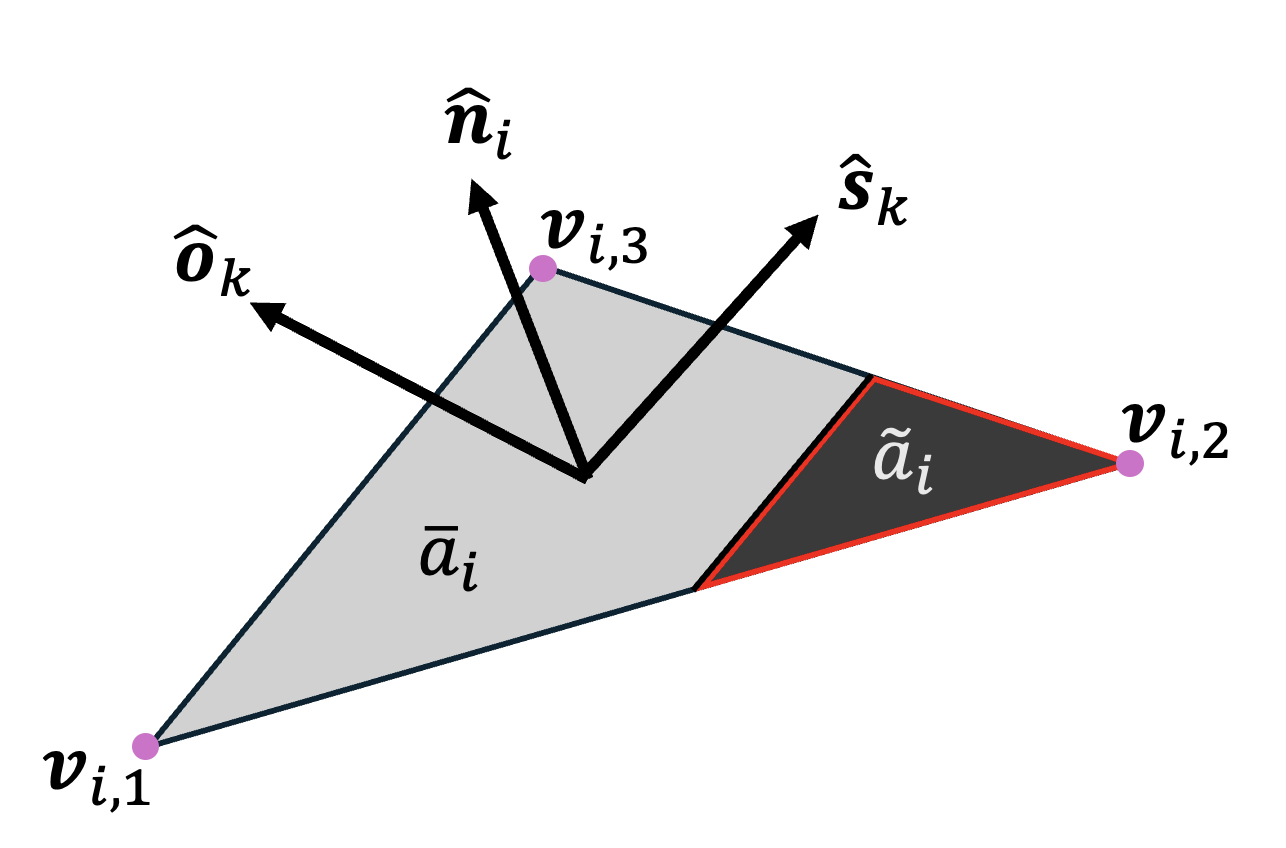
\includegraphics[width=\figmed]{obs_geom.png}
  \caption{Facet geometry including the observer direction $\unitv{o}$, Sun direction $\unitv{s}$, normal vector $\unitv{n}_i$, unshadowed area $\bar{a}_i$, shadowed area $\tilde{a}_i$, and counterclockwise vertex locations $\left\{ \vctr{v}_{i,1}, \vctr{v}_{i,2}, \vctr{v}_{i,3} \right\}$. }
  \label{fig:facet_geom}
\end{figure}

\begin{equation} \label{eq:us_area}
  \bar{a} = a - \sum_{d=1}^{n} \sum_{K \in \text{comb}(n,d)} (-1)^{d+1} A\left(\bigcap\limits_{k \in K} P_k\right).
\end{equation}

\begin{equation} \label{eq:brdf_blinn_phong}
  f_r(\unitv{s}, \unitv{o}) = \frac{C_d}{\pi} + \frac{n+2}{2\pi} \frac{C_s (\unitv{n} \cdot \unitv{h})^n}{4 (\unitv{n} \cdot \unitv{s})(\unitv{n} \cdot \unitv{o})}.
 \end{equation}

 \begin{equation} \label{eq:lc_norm}
  f_p(\unitv{s}_k, \unitv{o}_k) = \sum_{i=1}^n{\prf{B}\left[\bar{a}_i(\unitv{s}_k, \unitv{o}_k)
  f_{r,i}(\unitv{s}_k, \unitv{o}_k)
   (\unitv{n}_i \cdot \unitv{s}_k)
   (\unitv{n}_i \cdot \unitv{o}_k)
   \right]}. 
 \end{equation}

 \begin{equation} \label{eq:general_bright}
  \bar{S}_{\text{SO},k} = f_p(\unitv{s}_k, \unitv{o}_k) \frac{A \cdot \Delta t_k \cdot f_\odot(\vctr{r})}{g R_\oplus^2 r_k^2} \int_{0}^{\infty}{P(\lambda)Q(\lambda)T_k(\lambda) I_\odot(\lambda) \left(\frac{\lambda}{hc}\right)}\,d\lambda. 
\end{equation}

\begin{equation} \label{eq:sensor_noise}
  \sigma_\text{sensor} = \sqrt{n_\text{pix} \left( \Delta t \cdot \lambda_\text{dark} + \sigma_\text{read}^2 \right)}.
\end{equation}

\begin{equation}
  \sigma_\text{flat} = f_k \sqrt{\sum_{i=1}^{n_\text{pix}} S_i^2}.
\end{equation}

\begin{equation}
  \lambda_{\text{back},k} = n_{\text{pix},k} \left( \lambda_{\text{moon},k} + \lambda_{\text{star},k} + \lambda_{\text{twi},k} + \lambda_{\text{zod},k} + \lambda_{\text{star},k} + \lambda_{\text{poll},k} \right).
\end{equation}

\begin{equation} \label{eq:scint_noise}
  \sigma^2_{Y,k} = 10^{-6} D^{-4/3} (\Delta t)_k^{-1} \cos^{-3}\left(\gamma_k\right) e^{\frac{-2h_\text{obs}}{H}}.
\end{equation}

\begin{equation}
  \lambda_{\text{shot},k} = \frac{\bar{S}_{\text{SO},k}}{\sqrt{g}}.
\end{equation}

\begin{equation} \label{eq:sigma_total}
  \sigma^2_{S,k} = \lambda_{\text{back},k} + \bar{S}_{\text{SO},k} \sigma^2_{Y,k} + \lambda_{\text{shot},k} + \sigma^2_\text{flat},
\end{equation}

\begin{equation}
  S_{\text{SO},k} \sim \mathcal{N}\left( \bar{S}_{\text{SO},k}, \sigma^2_{S,k} \right).
 \end{equation}

 \begin{table}[ht]
  \centering
  \caption{Observation parameters 2}
  \vspace*{6pt}
  \begin{tabular}{|l|l|}
  \hline
  \textbf{Variable} & \textbf{Value} \\ \hline
  True inertia ratios $\begin{bmatrix}J_y / J_x & J_z / J_x\end{bmatrix}$ & $\begin{bmatrix} 1.0 & 0.5 \end{bmatrix}$ \\ \hline
  Initial simulation date & October 10, 2024 08:00:00.000 UTC \\ \hline
  Object identity (COSPAR ID) & 1987-084D \\ \hline 
 Light curve duration & $2$ minutes \\ \hline
 Measurement frequency & $0.5$ Hz \\ \hline
 Integration time & $0.01$ seconds \\ \hline
  \end{tabular}
  \label{tb:case1_in}
\end{table}

\begin{table}[ht]
  \centering
  \caption{Observation parameters 2}
  \vspace*{6pt}
  \begin{tabular}{|l|l|}
  \hline
  \textbf{Variable} & \textbf{Value} \\ \hline
  True inertia ratios $\begin{bmatrix}J_y / J_x & J_z / J_x\end{bmatrix}$ & $\begin{bmatrix} 1.0 & 0.5 \end{bmatrix}$ \\ \hline
  Initial simulation date & October 10, 2024 08:00:00.000 UTC \\ \hline
  Object identity (COSPAR ID) & 1987-084D \\ \hline 
 Light curve duration & $2$ minutes \\ \hline
 Measurement frequency & $0.5$ Hz \\ \hline
 Integration time & $0.01$ seconds \\ \hline
  \end{tabular}
  \label{tb:case1_in}
\end{table}

\section*{Acknowledgments}

people \cite{robinson2023}

\bibliography{cache/refs.bib}

% \begin{thebibliography}{}

% \bibitem{author73}
% Author T., (1973). Astrophysical Quantities, Athlone Press

% \bibitem{nobody97}
% Nobody B., Somebody G., Who D., et~al., (1997). {\it The book}, Publisher, ed. 2

% \bibitem{smith96}
% Smith A., Jones B., (1996). The new discovery, {\it Other Journal}, {\bf 223}(1), 1029--1101

% \end{thebibliography}
\end{document}
